%-----------------------------------------------------------------------------
%
%               Template for sigplanconf LaTeX Class
%
% Name:         sigplanconf-template.tex
%
% Purpose:      A template for sigplanconf.cls, which is a LaTeX 2e class
%               file for SIGPLAN conference proceedings.
%
% Guide:        Refer to "Author's Guide to the ACM SIGPLAN Class,"
%               sigplanconf-guide.pdf
%
% Author:       Paul C. Anagnostopoulos
%               Windfall Software
%               978 371-2316
%               paul@windfall.com
%
% Created:      15 February 2005
%
%-----------------------------------------------------------------------------


\documentclass[numbers]{sigplanconf}

% The following \documentclass options may be useful:

% preprint      Remove this option only once the paper is in final form.
% 10pt          To set in 10-point type instead of 9-point.
% 11pt          To set in 11-point type instead of 9-point.
% numbers       To obtain numeric citation style instead of author/year.

\usepackage{amsmath}
\newcommand{\cL}{{\cal L}}

\usepackage{url}
\usepackage[caption=false,font=normalsize,labelfont=sf,textfont=sf]{subfig}
\usepackage[nolist,nohyperlinks]{acronym}
\usepackage[table]{xcolor}
\usepackage[sharp]{easylist}

\hyphenation{op-tical net-works semi-conduc-tor a-na-ly-sis}

%glossaries package and acronym definitions
\usepackage{glossaries}
\setacronymstyle{long-short}
%\newacronym{frp}{FRP}{functional reactive programming}


\definecolor{mygreen}{rgb}{0,0.3,0}
\definecolor{myyellow}{rgb}{0.3,0.3,0}
\definecolor{mygrey}{rgb}{0.9,0.9,0.9}

\usepackage{listings}

\lstset{
    frameround=fttt,
    language=Java,
    numbers=left,
    numbersep=3pt,
    breaklines=true,
    breakatwhitespace=true,
    captionpos=b,
    keywordstyle=\color{blue}, 
    ndkeywordstyle=\color{purple},
    basicstyle=\scriptsize\ttfamily\color{black},
    numberstyle=\color{black},    
    stringstyle=\color{myyellow},
    commentstyle=\color{mygreen},
    backgroundcolor=\color{mygrey}
}

\usepackage{tikz}
\usetikzlibrary{shapes.multipart}

\begin{document}

\special{papersize=8.5in,11in}
\setlength{\pdfpageheight}{\paperheight}
\setlength{\pdfpagewidth}{\paperwidth}

\conferenceinfo{SOLA '06}{Darmstadt, Germany}
\copyrightyear{2016}
%\copyrightdata{978-1-nnnn-nnnn-n/yy/mm}%\copyrightdoi{nnnnnnn.nnnnnnn}

% Uncomment the publication rights you want to use.
%\publicationrights{transferred}
%\publicationrights{licensed}     % this is the default
%\publicationrights{author-pays}

\titlebanner{}        % These are ignored unless
\preprintfooter{footer}   % 'preprint' option specified.

\title{Language-independent Property Isolation in Tree-like Documents}
\subtitle{}

\authorinfo{Satia Herfert}
           {SOLA, TU Darmstadt}
           {satia.herfert@stud.tu-darmstadt.de}
           
\authorinfo{Jibesh Patra}
           {SOLA, TU Darmstadt}
           {jibesh.patra@gmail.com}
          
\authorinfo{Michael Pradel}
           {SOLA, TU Darmstadt}
           {michael@binaervarianz.de}

\maketitle

\begin{abstract}
le abstract
\end{abstract}

%\category{CR-number}{subcategory}{third-level}

% general terms are not compulsory anymore,
% you may leave them out
%\terms
%term1, term2

%\keywords
%keyword1, keyword2

\section{Introduction}
\label{sec_introduction}

\begin{easylist}[itemize]
# \textbf{Motivation}
## Debugging is time-consuming
## Isolating the cause of a bug in the input to a program is not easy. (Example: in a .c document as input to gcc)
## Smaller bug-reports for easier debugging and regression test cases
## Automation of the minimization desirable
# \textbf{Previous Work}
## Explain DD in one sentence
## Explain HDD~\cite{hdd} in one sentence
## HDD fails to restructure the tree and thus reduced documents are not minimal
# \textbf{Our approach}
## Build upon HDD and integrate tree transformations, not just subtree removal
## We identified templates of transformations, e.g. replacing a node with one of its children
## We learn where the template can be applied successfully from a corpus
## With this information we improve upon applying the template blindly to each node.
## After HDD has finished processing a level of the tree, we try to apply the transformation where applicable
## This approach is language-independent. The only language-specific parts are a conversion from code to tree and vice versa, and a large code corpus.
# \textbf{Evaluation}
## Tested with JS to minimize files that expose browser inconsistencies
## Tested with PY to minimize files that cause crashes in the interpreter
## We compared against DD and HDD and obtain files that are x\% smaller compared to HDD.
# \textbf{Contributions}
## List the main contributions
# \textbf{Paper outline}
## Explain outline of the paper
\end{easylist}

\section{Background}
\label{sec_background}

\begin{easylist}[itemize]
# \textbf{Delta Debugging}
## Input: Document to minimize and oracle
## Splits documents into tokens
## Tests subsets of the tokens with the oracle
## \textbf{Should we go into detail here or just redirect the reader to the paper?}
## Finds a local minimum (1-minimality)
## Disregards structure of the document, takes a lot of time/oracle invocations to finish
# \textbf{Hierarchical Delta Debugging}
## Can be applied to documents that have a tree representation, e.g. the AST of code
## Applies DD to each level of the tree successively. Removing a node of a level means removing the whole subtree
## HDD* repeats HDD until tree does not change any more
## Leverages the structure of the document to prune large parts of the input earlier.
## Therefore, outperforms DD.
## Can only delete nodes from the tree, not restructure them
## Results in reduced trees that can be minimized further
## Examples: IfStatement and BinaryExpression
\end{easylist}

\section{Our Approach}
\label{sec_approach}

\begin{easylist}[itemize]
# \textbf{Transformation templates}
## Instead of blindly trying different transformations in a tree, we define transformation templates.
## These templates were obtained by analyzing documents that were minimized with HDD and conclude what transformation would be necessary to further reduce the tree, maintaining the desired property.
## As different trees (e.g. JS AST) have particular rules, how a tree may be structured, a transformation might not always be applicable.
## Applying it anyhow would result in a tree that cannot be converted to code.
## Example: IfStatement $-test->$ UnaryOperator is not a valid tree
## We learn when a transformation can be applied by analyzing a large code corpus.
## $applicable(T, C)$ for a template and its configuration tells if it can be applied

# \textbf{Actual templates}
## Template 1: Child substitution
### A node is replaced with one of its children.
### Configuration: Node label N, Parent label P, ingoing edge label e1, child label C
### This transformation can be applied for $P-e1->N-e2->C$, iff $P-e1->C$ is also a valid subtree.
### While analyzing the code corpus, for each particular node label L we collect a set S of pairs (P,e) that appeared as the parent node and the ingoing edge to the node with label L.
### Before applying "Child substitution" to a node N with a child C, we check if the tuple (P,e) of N's parent node and ingoing edge appears in the set S of C.
## Template 2: \textbf{Think of something cool here}

# \textbf{Algorithm: Transformation-aware HDD (TA-HDD)}
## As in HDD, apply DD to a whole level of a tree
## For each template T, for each applicable configuration tuple C
### With the gathered information, test if $applicable(T, C)$ is true. If so, apply the transformation.
### Test if $oracle(tree) == fail$ (meaning the property holds). In that case, leave the transformation, and include the new node in the testing of the current level. Otherwise, undo the transformation.
# \textbf{TA-HDD*}
## As in HDD, applying a transformation to a lower level might enable removing or transforming a node in a higher level of the tree. Give an example.
## Just like HDD*, we repeat TA-HDD until the tree ceases to change, to account for that problem.

# \textbf{Tailoring the algorithm to a specific language}
## This approach is language-independent. The only language-specific parts are a conversion from code to tree and vice versa, and a large code corpus.
\end{easylist}

\section{Evaluation}
\label{sec_evaluation}

\begin{easylist}[itemize]
# \textbf{Experiment setup}
## JS inconsistencies
### 44 files. Oracle: they expose an inconsistency across browsers
### Used Firefox 25 vs Chrome 48
### An inconsistency means: One browser throws an exception and the other does not; they throw different exceptions; they have different read-write traces as collected with jalangi.
## PY crashes
### 10 files. Oracle: they crash the python interpreter with a segmentation fault or stack overflow (result.status == 134 or result.status == 139)
### Used V2.7.6 and V3.4.3, and actual bug reports. (Put a table)
\end{easylist}

\begin{easylist}[itemize]
# \textbf{Is the code base that we analyze large enough to learn sufficient information for the transformation templates?}
## JS corpus with nearly 140,000 files
## See Figure \ref{fig_learning-graph-js}
## Even after analyzing such a large code corpus, new transformations are still identified occasionally.
## But the curve flattens out, suggesting that \emph{enough} transformations were identified to account for a large portion oF JS code.
\end{easylist}

\begin{figure}
\begin{center}
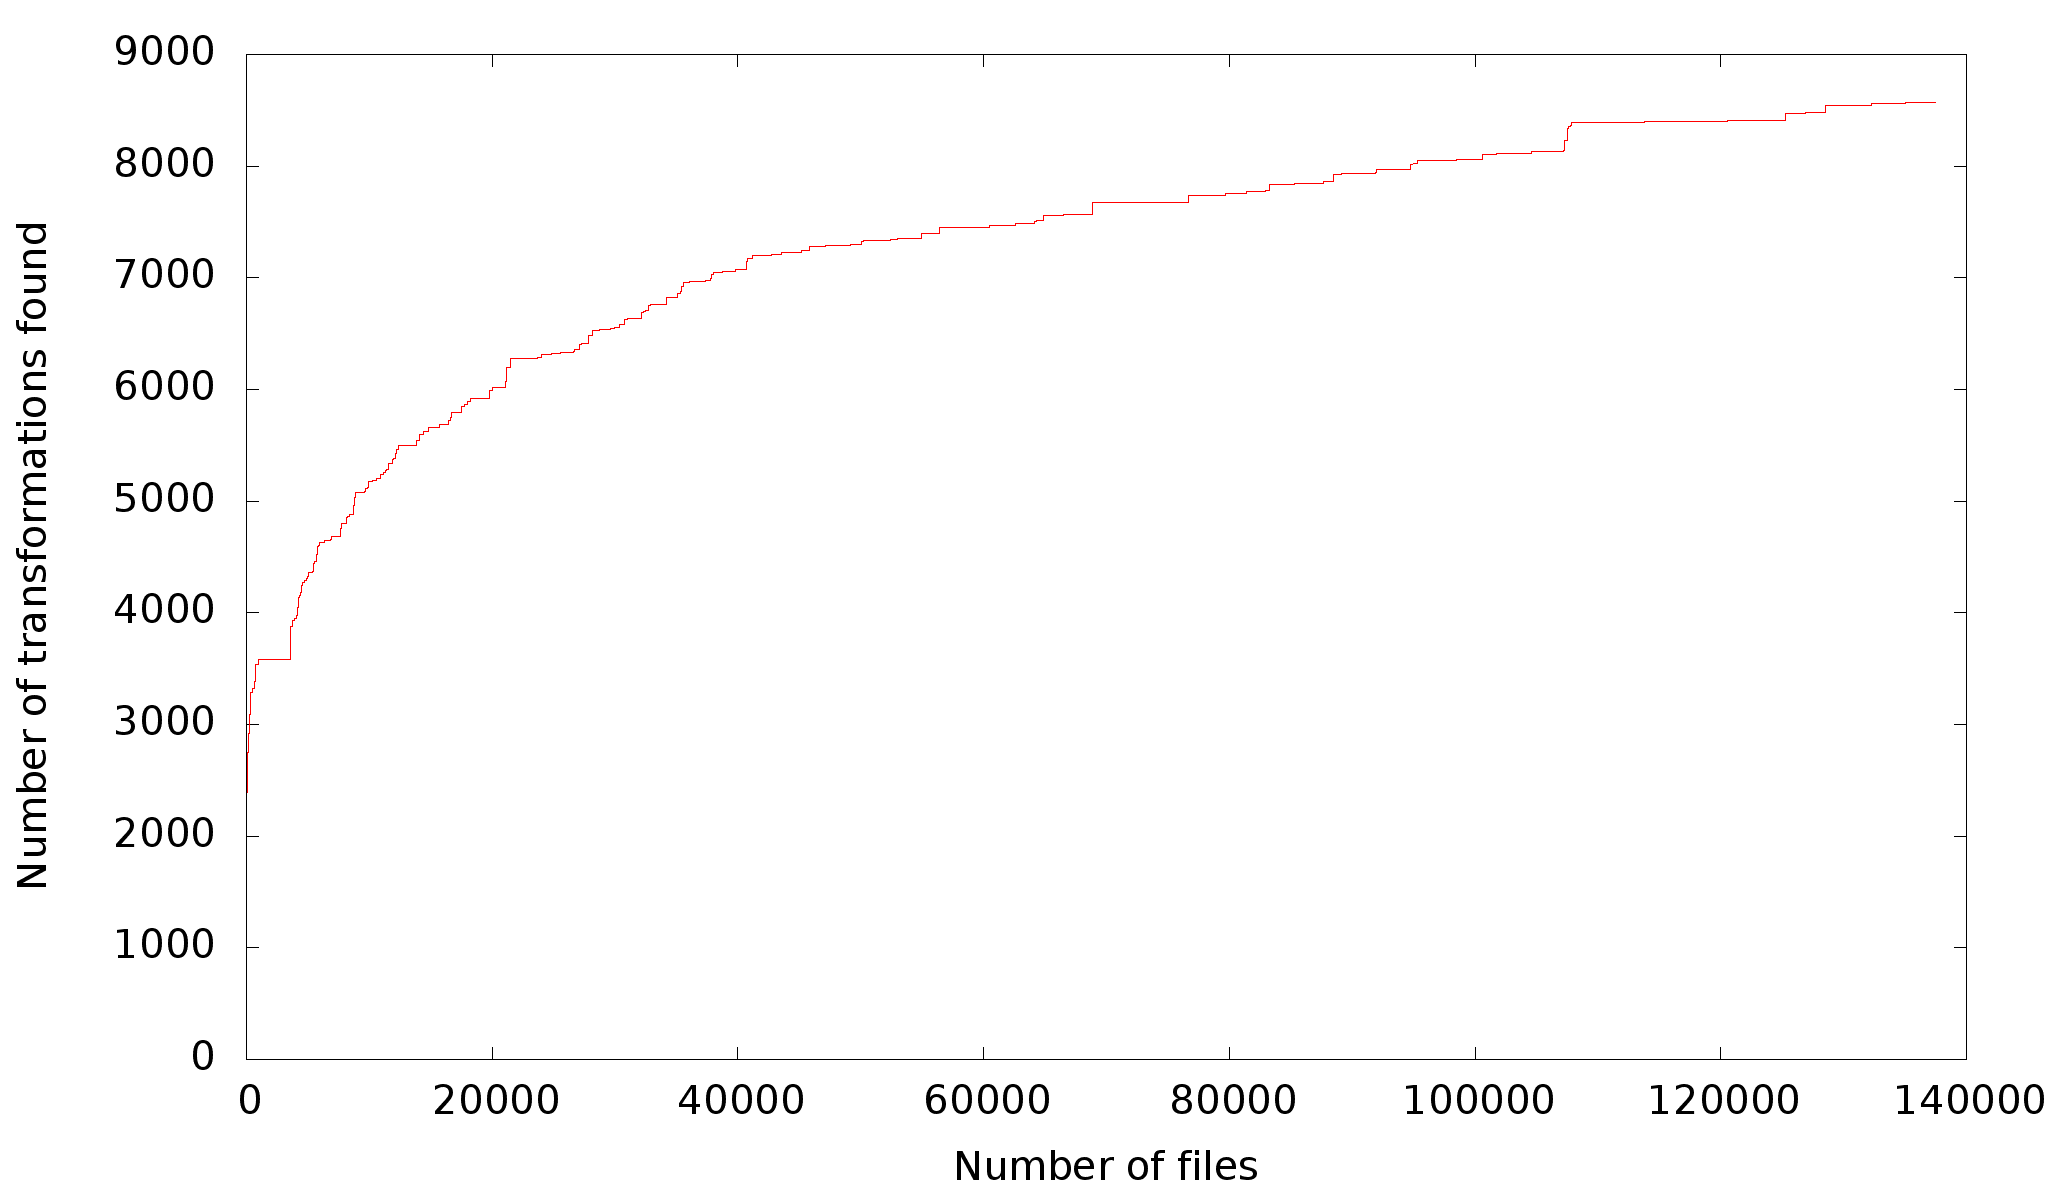
\includegraphics[width=\columnwidth]{img/learning-graph-js.png}
\end{center}
\caption{Learning curve for JS corpus.}
\label{fig_learning-graph-js}
\end{figure}

\begin{easylist}[itemize]
# \textbf{Is it worth analyzing a code corpus and only trying transformations when we think they are applicable?}
## With the above experiment setup, we compared resulting file size, number of oracle invocations and time taken for TA-HDD vs TA-HDD that blindly skips the test $applicable$.
## Size is ca the same, skipping the test results in ca 50 \% more tests/time.
## Also see Figure \ref{fig_comparison}.
\end{easylist}

\begin{easylist}[itemize]
# \textbf{How does our approach compare to other algorithms in terms of resulting file sizes, number of oracle invocations, and time taken to minimize a file?}
## With both JS and PY the experiment was conducted with DD char-based, DD line-based, HDD, HDD*, TA-HDD, TA-HDD*
## Results can be seen in Figure \ref{fig_comparison}.
## Size is ca 1/3 of HDD
## Tests is comparable to HDD (little less)
## Time is comparable to HDD (little less)
\end{easylist}

\begin{figure*}
\begin{center}
\subfloat[Comparing size \label{fig_comparison-size}]{%
  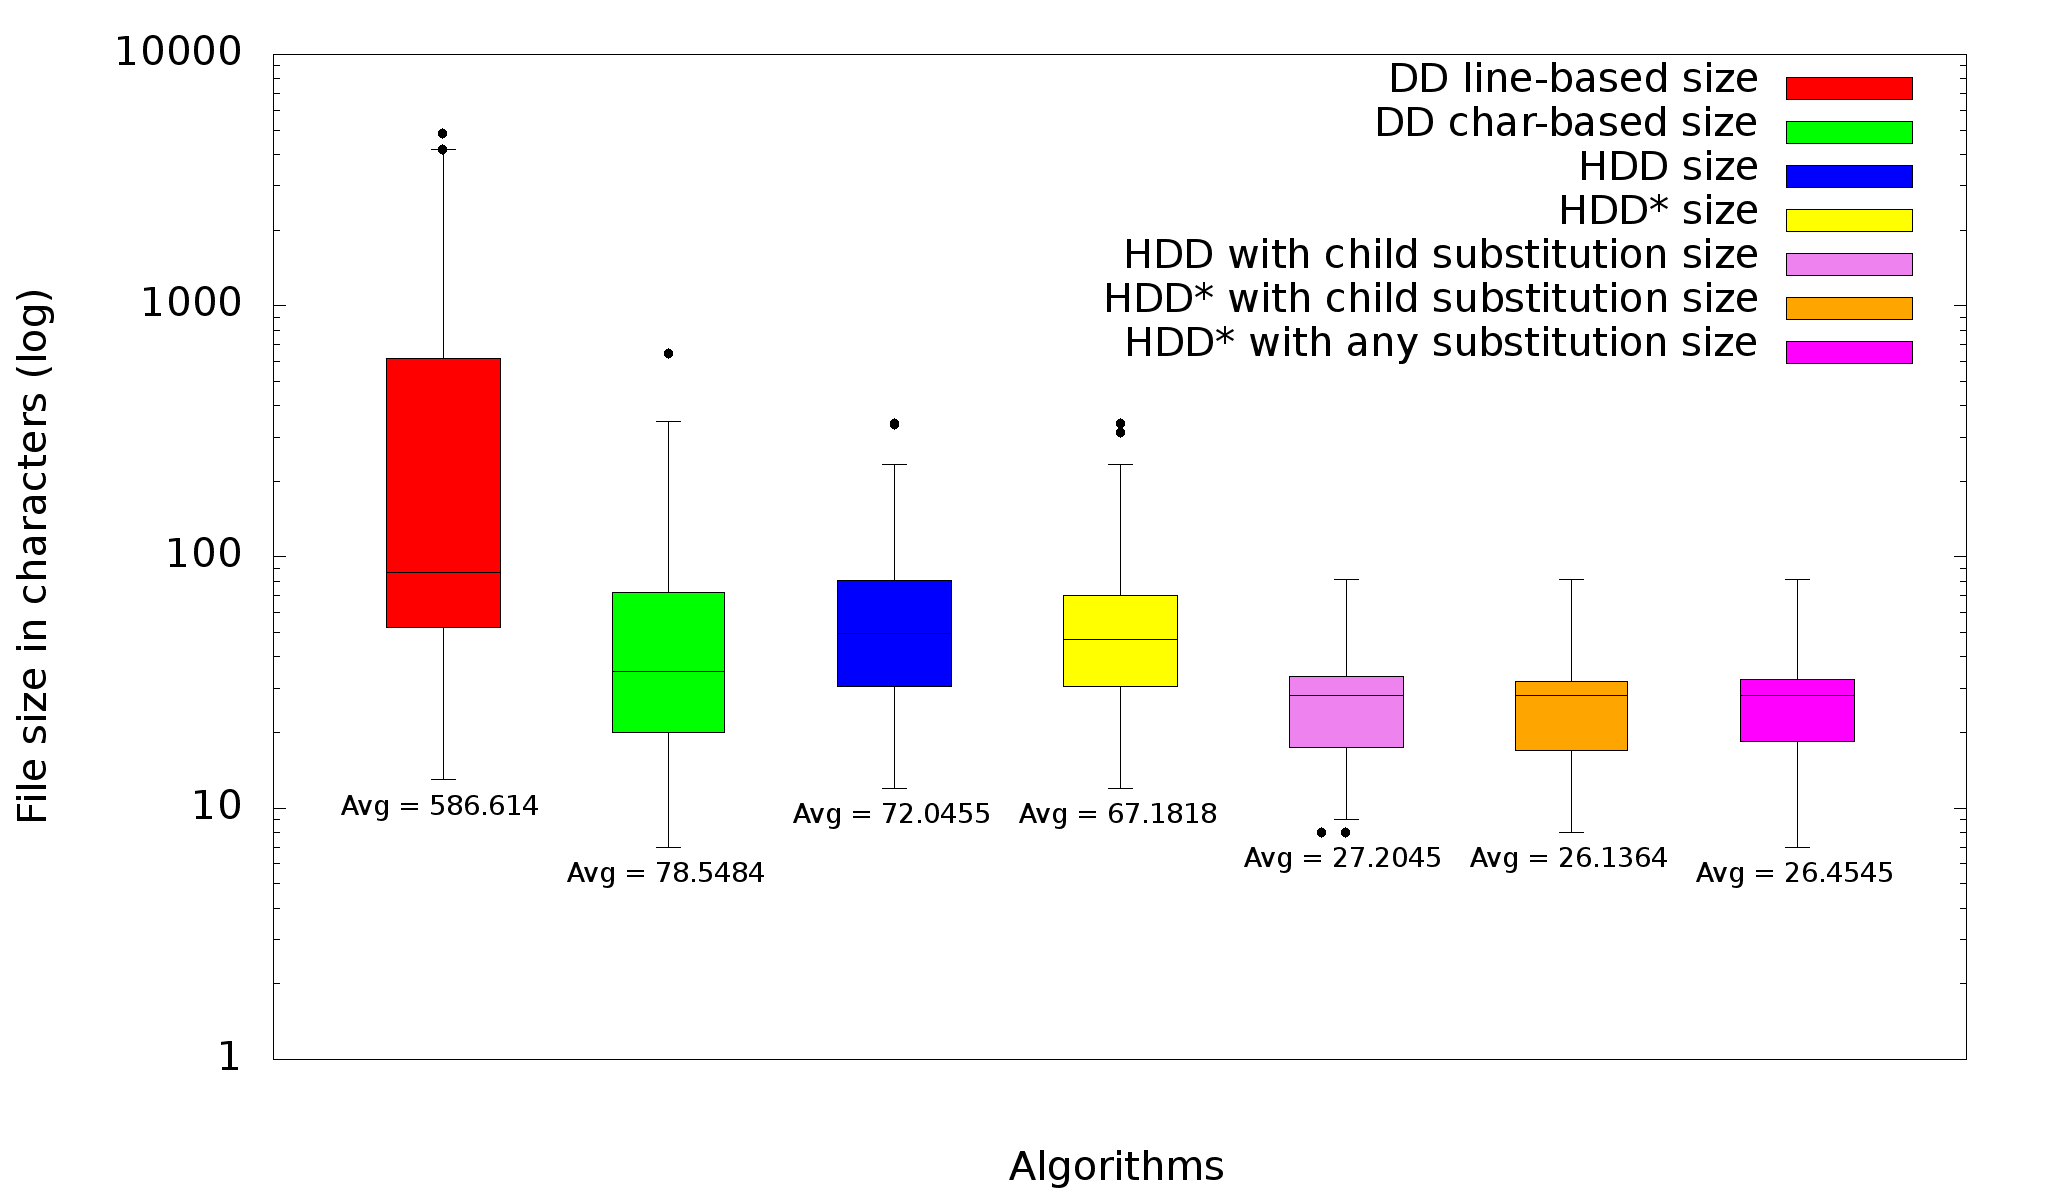
\includegraphics[width=0.6\textwidth]{img/box-size-js.png}
}
\\
\subfloat[Comparing tests \label{fig_comparison-tests}]{%
  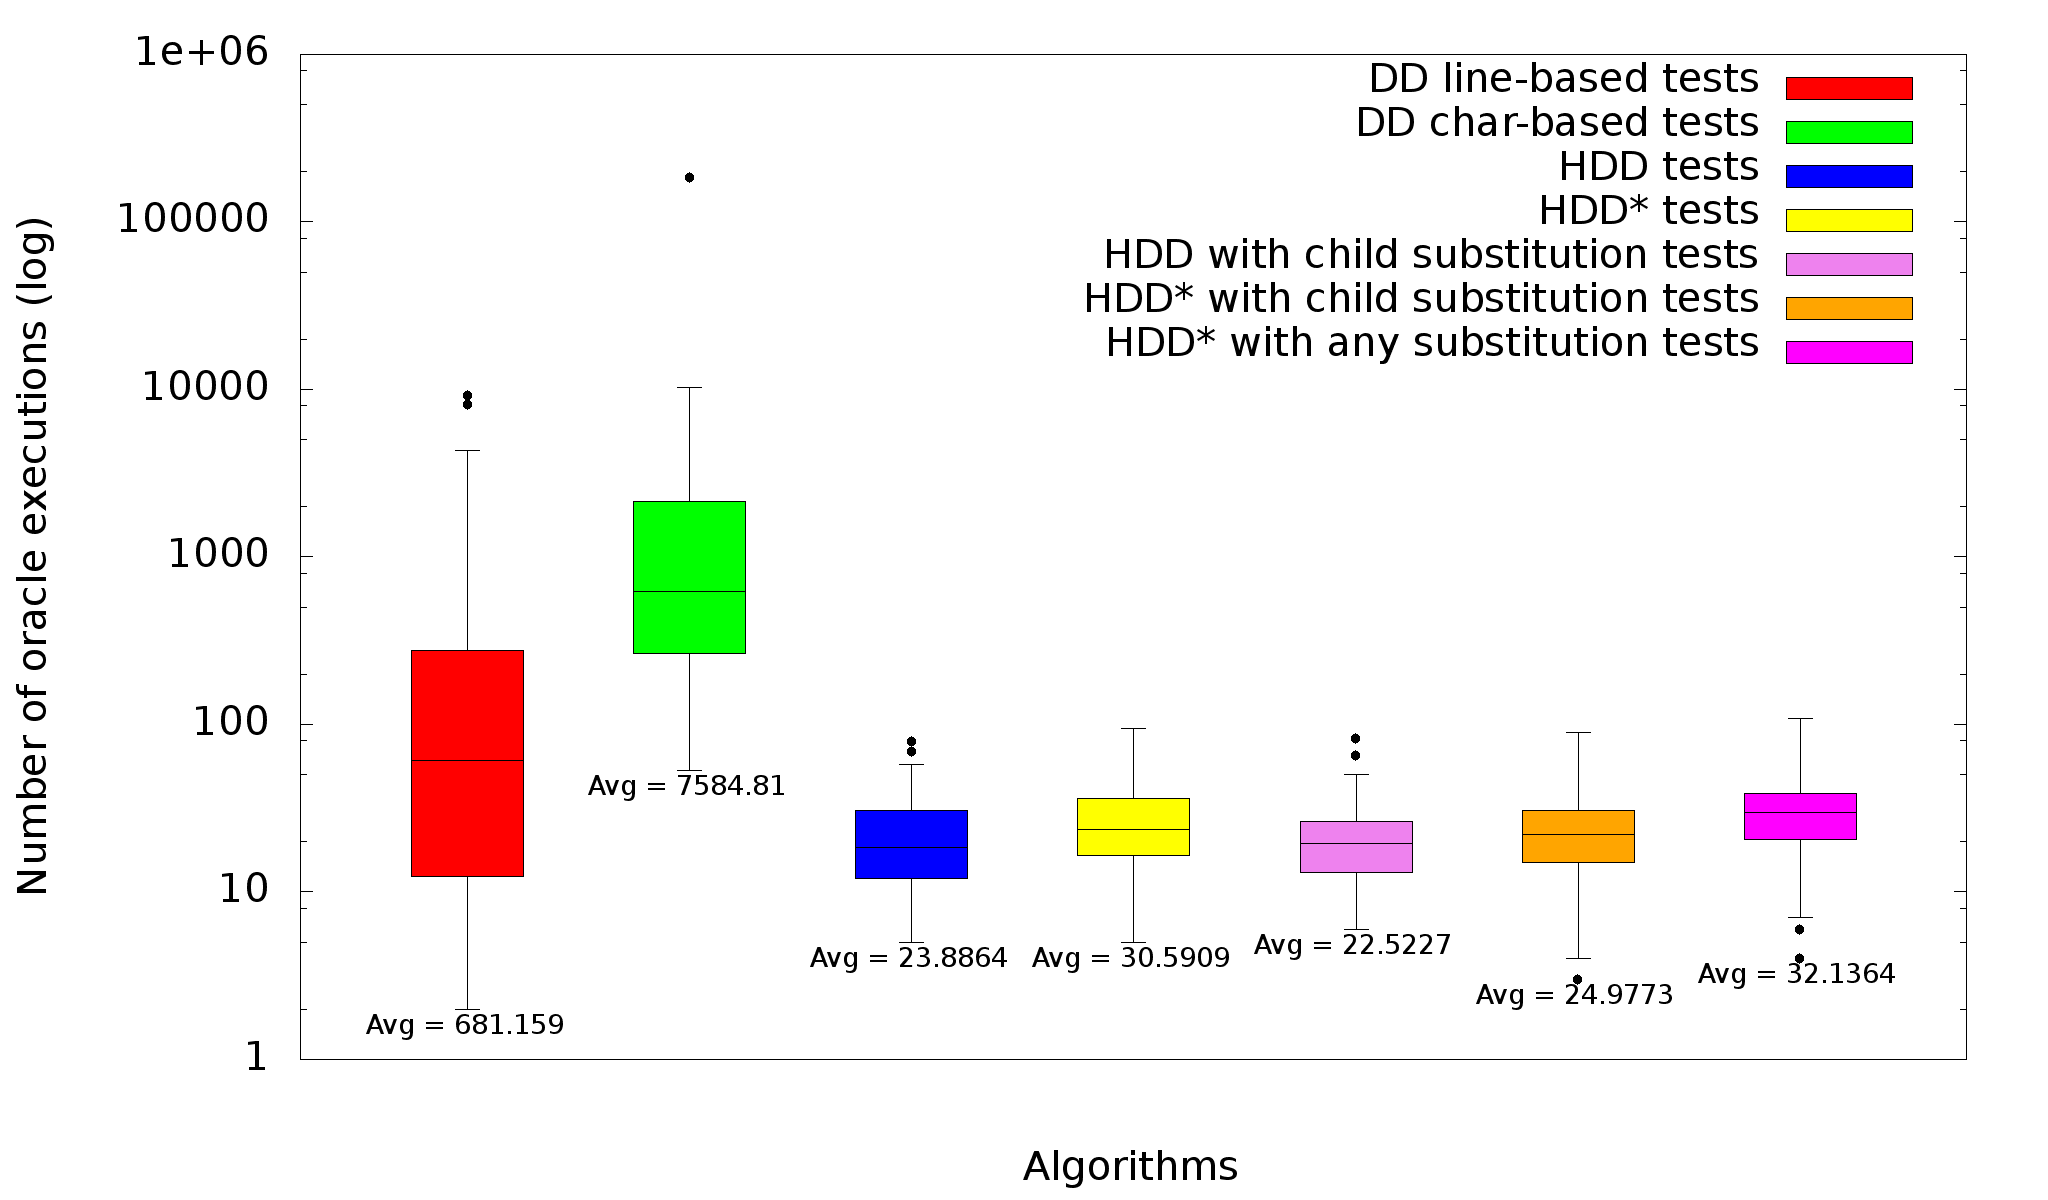
\includegraphics[width=0.6\textwidth]{img/box-tests-js.png}
}
\\
\subfloat[Comparing time \label{fig_comparison-time}]{%
  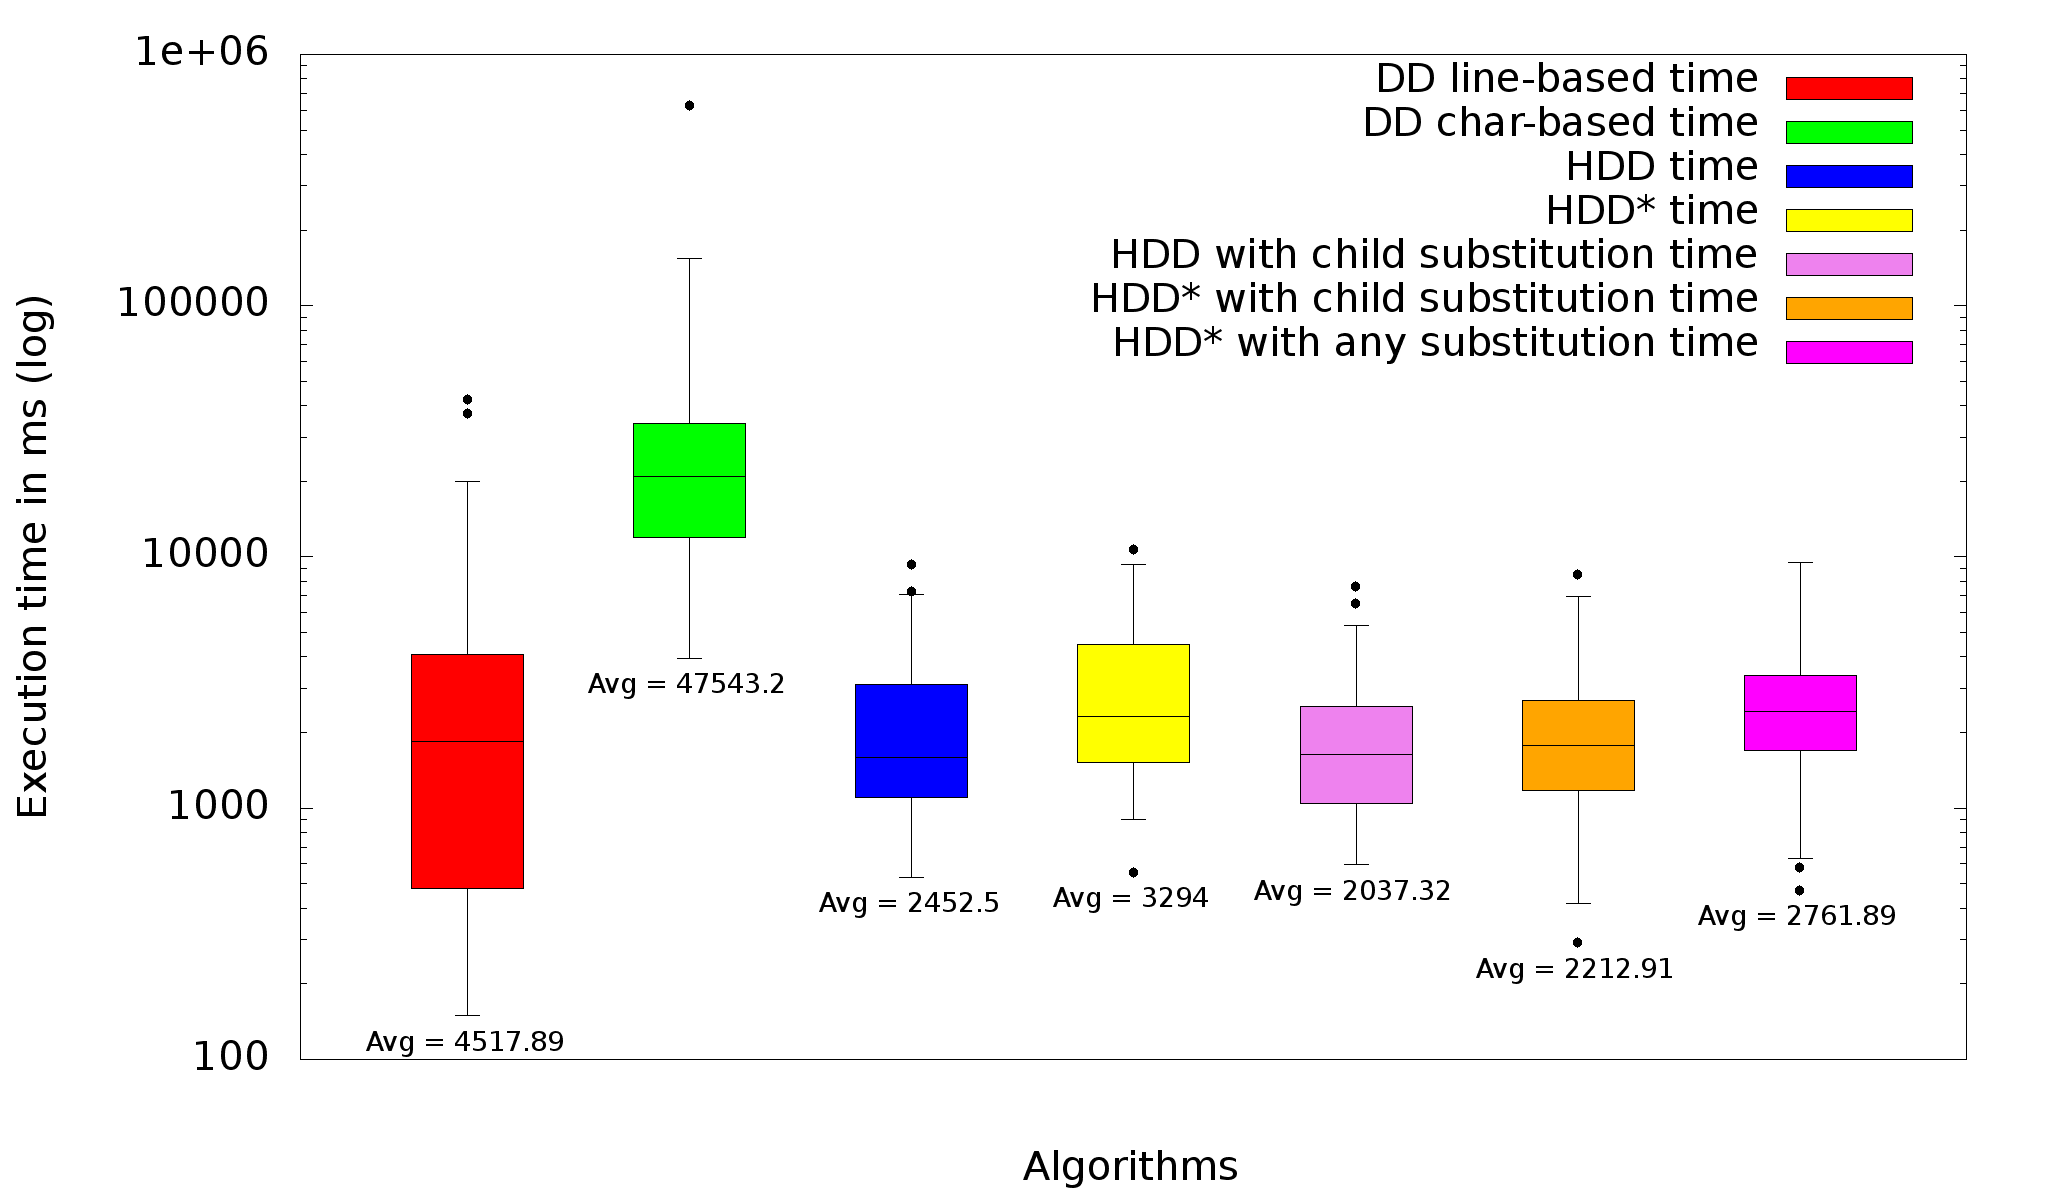
\includegraphics[width=0.6\textwidth]{img/box-time-js.png}
}
\end{center}
\caption{Comparing file sizes, tests, and time for JS.}
\label{fig_comparison}
\end{figure*}

\section{Related work}
\label{sec_related-work}

\section{Conclusion}
\label{sec_conclusion}

\begin{easylist}[itemize]
# We spot weaknesses in HDD: It fails to transform trees
# We identify different transformations that reduce minimized files further
# We define transformation templates with the above information
# We learn information from a large code corpus to define when a transformation is applicable
# We design a new algorithm that incorporates transformations into HDD
# We outperform HDD in terms of resulting file size without needing more time
\end{easylist}

% We recommend abbrvnat bibliography style.
\bibliographystyle{plainnat}
\bibliography{bibliography}

\end{document}